\chapter{Results and Discussion}

Here we examine both the performance and visual quality of our global illumination algorithm. The primary means of evaluating performance is based on frame time. The times of each render pass are recorded as well as a total frame time. Evaluating visual quality is based largely on whether the lighting appears smooth and believable with a minimal amount of noise and artifacts.

We also discuss the application of voxel warping and how it compares with other global illumination methods. Unfortunately, direct performance and visual quality comparisons are difficult to objectively measure as there are many contributing factors---mesh complexity and optimizations, texture resolution and format, shading model, graphics API, hardware, GPU driver version, and more---that affect the final comparison, in addition to the exact implementation details. Nevertheless, we provide motivations and tradeoffs between our method and others and their potential impact on performance and quality.

\section{Test Setup}
% TODO verify driver, kernel, resolution when getting final results
All results are obtained from a system with an i5-2400 CPU, 8GB of DDR3 RAM, and an NVIDIA GeForce GTX 970 GPU. The system is running Arch Linux kernel 4.16.8-1 and uses the proprietary NVIDIA graphics driver version 396.24. The application uses an OpenGL 4.5 context and the scene is rendered with a window resolution of 1920x1080.

% TODO give #vertices, texture resolutions and sizes?
The model used in the test scenes is the Crytek Sponza scene\footnote{The original Sponza model can be acquired from Crytek~\cite{sponza_og}. The model we use is modified by Alexandre Pestana~\cite{sponza_pbr}.}. The textures from the original Sponza scene are replaced with ones necessary for physically-based rendering (materials are defined by a diffuse color, roughness, metallic coefficient, normal, and optionally an alpha texture). Mipmaps for the original textures were also precomputed and stored along with the full size 1024x1024 textures as DDS (Microsoft DirectDraw Surface) files using the compressed DXT5 format for faster scene loading.

To measure performance timings for each render pass we make use of OpenGL timer queries using the \verb#GL_TIME_ELAPSED# query type. The results of the query object are double buffered to ensure introducing the timer query does not affect the total render time.

Unless otherwise mentioned, voxel resolutions are 256x256x256 with 6 mipmap levels.

\section{Analysis}
In the following sections we evaluate various aspects of our work. First, we discuss the global illumination algorithm as a whole. Second, we compare the rasterization-based and tessellation-based voxelization algorithms. Lastly, we provide the results of our voxel warping and some insights on future improvements.

\subsection{Global Illumination}
We test the algorithm with different screen resolutions and voxel grid resolutions. The rendered images with different voxel grid resolutions are shown in Figure~\ref{fig:results_rendered}. We see that the main difference with different voxel grid resolutions is how far the light spreads due to the larger voxels.

Table~\ref{tbl:renderpasstiming} shows timing results from the complete global illumination algorithm and Figure~\ref{fig:renderpasstiming} plots the data as a stacked bar chart. Recall that a minimum goal for real-time is 30 frames per second and a target is 60 frames per second, which correspond to individual frame times of 33.3ms and 16.7ms, respectively. We see that the total frame time always meets the goal of 60 frames per second.

The data shows that shadowmap creation and radiance injection was independent of screen resolution and voxel resolution\footnote{As expected, since the main factor for both of these render passes is the size of the shadowmap, which remained constant at 4096x4096.}. The voxelization and radiance filtering steps both only depended on voxel grid resolution. The depth prepass also only varied with respect to screen resolution. The final shading predictably depended on both voxel grid resolution and screen resolution. However, larger voxel grid resolutions did not affect the final shading times by much at a given screen resolution, with approximately a 1.5ms difference between using a voxel resolution of 64 versus 256. Ultimately, the time spent for the shading dominates all other render passes and thus makes itself a prime target for any future work on optimizing for speed.

\begin{figure}
\centering
\begin{subfigure}[t]{0.475\textwidth}
    \adjincludegraphics[width=0.95\textwidth,trim={0 {0.1\height} {0.25\width} 0},clip]{results_720_64}
    \caption{}
\end{subfigure}
~
\begin{subfigure}[t]{0.475\textwidth}
    \adjincludegraphics[width=0.95\textwidth,trim={0 {0.1\height} {0.25\width} 0},clip]{results_720_128}
    \caption{}
\end{subfigure}

\begin{subfigure}[t]{0.475\textwidth}
    \adjincludegraphics[width=0.95\textwidth,trim={0 {0.1\height} {0.25\width} 0},clip]{results_720_256}
    \caption{}
\end{subfigure}
\caption{The scene rendered with voxel grid resolutions of $64^3$, $128^3$, and $256^3$.}
\label{fig:results_rendered}
\end{figure}

\begin{table}
\centering
\small
\begin{tabular}{l ccc ccc ccc}
\toprule
Render Pass & \multicolumn{9}{c}{Render Pass Time (ms)} \\
& \multicolumn{3}{c}{1280x720} & \multicolumn{3}{c}{1600x900} & \multicolumn{3}{c}{1920x1080} \\
& 64 & 128 & 256 & 64 & 128 & 256 & 64 & 128 & 256 \\
\midrule
Voxelize           & 0.90 & 1.13 & 2.40  & 0.70 & 1.12 & 2.39  & 0.72 & 1.15 & 2.41\\
Shadowmap          & 0.69 & 0.69 & 0.69  & 0.69 & 0.69 & 0.69  & 0.68 & 0.68 & 0.69\\
Radiance Injection & 0.92 & 0.92 & 0.93  & 0.92 & 0.92 & 0.93  & 0.92 & 0.92 & 0.93\\
Radiance Filtering & 0.04 & 0.10 & 0.55  & 0.05 & 0.10 & 0.56  & 0.04 & 0.10 & 0.55\\
Depth Prepass      & 0.20 & 0.20 & 0.20  & 0.25 & 0.26 & 0.25  & 0.31 & 0.31 & 0.36\\
Final Shading      & 3.89 & 4.81 & 5.32  & 5.98 & 6.42 & 7.10  & 8.23 & 9.40 & 9.75\\
\midrule
Total              & 7.02 & 8.21 & 11.12  & 9.46 & 10.15 & 13.43  & 11.23 & 12.83 & 16.31\\
\bottomrule
\end{tabular}
\caption{Times measured for each render pass for various screen resolutions and voxel grid resolutions. The total timer also accounts for any other operations performed within each frame (i.e.\ the sum of the render pass times is not necessarily the complete time for an entire frame). Voxelization is done using the tessellation-based approach.}
\label{tbl:renderpasstiming}
\end{table}

\begin{figure}
\centering
\pgfplotstableread[row sep=\\]{
    Resolution Voxelize Shadowmap Inject Filter Shading Other\\
    720p64 0.90  0.69  0.92  0.04  4.19 0.38\\
    720p128 1.13  0.69  0.92  0.10  5.01 0.36\\
    720p256 2.40  0.69  0.93  0.55  5.52 1.03\\
    900p64 0.70  0.69  0.92  0.05  6.23 0.87\\
    900p128 1.12  0.69  0.92  0.10  6.68 0.64\\
    900p256 2.39  0.69  0.93  0.56  7.35 1.51\\
    1080p64 0.72  0.68  0.92  0.04  8.54 0.33\\
    1080p128 1.15  0.68  0.92  0.10  9.71 0.27\\
    1080p256 2.41  0.69  0.93  0.55  10.01 1.62\\
}\dataset
\begin{tikzpicture}[scale=0.9]
    \begin{axis}[nodes near coords ybar stacked configuration/.style={},ybar stacked, symbolic x coords={720p64, 720p128, 720p256, 900p64, 900p128, 900p256, 1080p64, 1080p128, 1080p256}, xtick=data, xticklabel style={rotate=45}, legend style={at={(1.05,0.5)}, anchor=west}, xlabel={Screen Resolution x Voxel Grid Size}, ylabel={Time (ms)}, enlarge y limits={0.2, upper}, title={Frame Times}, ymin=0, xlabel near ticks, xmajorticks=false]
    \addplot table[meta=Resolution, y=Voxelize] \dataset;
    \addplot table[meta=Resolution, y=Shadowmap] \dataset;
    \addplot table[meta=Resolution, y=Inject] \dataset;
    \addplot table[meta=Resolution, y=Filter] \dataset;
    \addplot table[meta=Resolution, y=Shading] \dataset;
    \addplot[point meta=y, nodes near coords, nodes near coords align={above}, nodes near coords style={/pgf/number format/.cd, fixed zerofill, precision=1}] table[meta=Resolution, y=Other] \dataset;

    \legend{Voxelize, Shadowmap, Radiance Injection, Radiance Filtering, Final Shading, Other}
    \end{axis}
\end{tikzpicture}
\caption{Graph showing the render pass times. Each bar shows the relative time contributions of each render pass. The depth prepass is incorporated into the Final Shading category and the Other category accounts for any other miscellaneous tasks done while rendering the frame.}
\label{fig:renderpasstiming}
\end{figure}

\subsection{Tessellated Voxelization}
The result of shading the scene with both voxelization methods is shown in Figure~\ref{fig:voxelcomparison}. First, we notice the rasterized approach generates `smoother' voxels. This is a result of the rasterization discretizing the fragments as well as possibly not generating fragments for small triangles. The tessellated approach, since it uses the raw vertex positions to compute the voxel position, does not exhibit this smoothing effect. Also, with the rasterized approach we see cracks on the archs from imperfect conservative rasterization. The tessellated approach does not have issues with conservative rasterization. Instead, the issue is with large triangles (such as the floor): the GPU has a maximum supported tessellation level. Triangles that require a higher tessellation level than this hardware maximum will end up having holes\footnote{A possible workaround for this would be to subdivide large triangles before voxelizing, such as when loading in the mesh.}.

In terms of both performance and visual quality both voxelization methods are very similar. Voxelization times for each method are shown in Table~\ref{tbl:voxelizationtiming} and graphed in Figure~\ref{fig:voxelizationtiming}, where we see the tessellation-based voxelization is slightly slower than the rasterization-based approach\footnote{However both implementations were not heavily optimized.}. Figure~\ref{fig:results_voxelization} compares the final rendered scene with both voxelization methods. The differences are minor.

Another limitation specific to the rasterized approach is shown in Figure~\ref{fig:voxellimitations}. The fragment resolution must be set appropriately for the voxel density\footnote{This is especially important for the warped voxelization approaches, since the density is not uniform}. The tessellated voxels do not suffer from this issue since we do not rely on the rasterizer to produce fragments.

Ultimately, both voxelization methods are sufficient for real-time global illumination. The (unoptimized) tessellation-based approach is slightly easier to implement and debug\footnote{Since the voxels are written in the tessellation evaluation stage, it is simple to add a geometry shader that takes the vertices and expands them into cubes, which are then rasterized and shaded with the vertex color (the same color inserted into the voxel texture).} but is slower than the rasterization-based approach. % One benefit of the tessellation-based approach is the voxel positions are continuous, unlike the rasterized voxels which are fixed at discrete positions according to the viewport resolution. This eliminates having to deal with cracks caused by higher density areas. (instead the limitation is on # of tesslevels ...)

\begin{figure}
\begin{subfigure}[t]{0.475\textwidth}
    \adjincludegraphics[width=\textwidth,trim={0 0 {0.25\width} 0},clip]{rastervoxel_nowarp}
    \caption{Rasterized voxels}
\end{subfigure}
~
\begin{subfigure}[t]{0.475\textwidth}
    \adjincludegraphics[width=\textwidth,trim={0 0 {0.25\width} 0},clip]{tessvoxels_nowarp}
    \caption{Tessellated voxels}
\end{subfigure}
\caption{Comparison between the scene shaded based on the rasterized voxels (left) and the tessellated voxels (right).}
\label{fig:voxelcomparison}
\end{figure}

\begin{figure}
\centering
\begin{subfigure}[t]{0.475\textwidth}
    \adjincludegraphics[width=\textwidth,trim={0 0 {0.25\width} 0},clip]{rasterlimited}
    % \caption{Rasterized voxels}
\end{subfigure}
% ~
% \begin{subfigure}[t]{0.475\textwidth}
%     \adjincludegraphics[width=\textwidth,trim={0 0 {0.25\width} 0},clip]{tesslimited}
%     \caption{Tessellated voxels}
% \end{subfigure}
% \caption{Images showing the main limitations of each voxelization method. For the rasterized approach (left), the fragment resolution must be large enough for a particular voxel density. For the tessellated approach (right), cracks appear if a higher tessellation level than the hardware supported maximum is required.}
\caption{Image showing a limitation of the rasterized approach: the fragment resolution must be large enough for a particular voxel density. Otherwise, cracks will occur in the final voxelization.}
\label{fig:voxellimitations}
\end{figure}

\begin{figure}[h!]
\centering
    \begin{subfigure}[t]{0.475\textwidth}
        \adjincludegraphics[width=\textwidth,trim={0 0 {0.25\width} 0},clip]{results_voxelraster}
        \caption{Rasterized voxels}
    \end{subfigure}
    ~
    \begin{subfigure}[t]{0.475\textwidth}
        \adjincludegraphics[width=\textwidth,trim={0 0 {0.25\width} 0},clip]{results_voxeltess}
        \caption{Tessellated voxels}
    \end{subfigure}
    \caption{The final rendered image for both voxelization methods have negligible visual differences.}
    \label{fig:results_voxelization}
\end{figure}

\begin{figure}
\centering
\pgfplotstableread[row sep=\\]{
    Resolution Rasterized Tessellated\\
    64         0.53       0.70\\
    128        0.85       1.12\\
    256        1.91       2.35\\
}\dataset
\begin{tikzpicture}[scale=0.9]
    \begin{axis}[ybar=5pt, symbolic x coords={64,128,256}, xtick=data, legend style={at={(1.05,0.5)}, anchor=west}, xlabel={Voxel Grid Size}, ylabel={Time (ms)}, enlarge y limits={0.2, upper}, enlarge x limits={0.2}, title={Voxelization Time},nodes near coords, nodes near coords align={above}, nodes near coords style={/pgf/number format/fixed}, ymin=0, ybar=10pt, xtick align=inside, xmajorticks=false]
    \addplot table[meta=Resolution, y=Rasterized] \dataset;
    \addplot table[meta=Resolution, y=Tessellated] \dataset;

    \legend{Rasterized, Tessellated}
    \end{axis}
\end{tikzpicture}
\caption{Graph comparing the voxelization time for both approaches at different voxel grid sizes.}
\label{fig:voxelizationtiming}
\end{figure}

\begin{table}[H]
\centering
\small
\begin{tabular}{lcc}
\toprule
\multirow{2}{*}{Voxel Grid Size} & \multicolumn{2}{c}{Voxelization Time (ms)} \\
& Rasterization-Based & Tessellation-Based \\
\midrule
64x64x64        & 0.53 & 0.70\\
128x128x128     & 0.85 & 1.12\\
256x256x256     & 1.91 & 2.35\\
\bottomrule
\end{tabular}
\caption{Time spent voxelizing the scene with varying voxel grid resolutions. For the rasterization-based approach the MSAA method of conservative rasterization is used.}
\label{tbl:voxelizationtiming}
\end{table}

\subsection{Integration of Voxel Cone Tracing into Existing Engines}
Voxel cone tracing is an attractive method for adding full global illumination to existing engines. The necessary information needed for the algorithm should already be available in most engines. A voxelized representation of the scene can be generated from any arbitrary triangle mesh using either of the voxelization methods presented. Other methods for voxelization could also be used if, for example, some geometry is generated procedurally. For radiance injection the only external inputs required are shadowmaps (or RSMs) for any lights that will contribute to the indirect lighting. Finally, the cone tracing needs surface normals and a TBN matrix (to transform the cone directions to world space), which will already be available for any engine which supports normal mapping.

\subsection{Voxel Warping}
Recall that the goal of voxel warping is to achieve a nonuniform voxel density. Ideally, this results in finer lighting detail for those areas that have increased density. Other approaches to increasing voxel resolution include clipmaps and octrees, as discussed in the Related Works. Fundamentally, however, the voxel resolutions were restricted to fixed sizes. With voxel warping we investigated how lifting this restriction would affect the voxelization quality.

The first method of voxel warping used a warp function to adjust the voxel density based on distance from the camera. Figure~\ref{fig:results_warpslope} shows a visual representation of the density. The effect of the warping on the final lighting is fairly minimal, as seen in Figure~\ref{fig:results_voxelwarp}. The big problem with voxel warping arises when the camera moves, since the continuously changing resolution causes voxels to flicker as they move throughout the voxel grid. Typically when the voxel sizes are all uniform this is fixed by snapping the voxel grid to discrete steps; but, with voxel warping, there is no single step size appropriate for all voxels.

\begin{figure}[h!]
    \centering
    
\includegraphics[width=0.5\textwidth]{voxelwarp_slope.png}
    \caption{The scene is colored based on its density along the x axis (derived from the gradient of the warp function). Blue tints correspond to a slope of 2 and green corresponds to a slope of 1 (same as no warping).}
    \label{fig:results_warpslope}
\end{figure}

\begin{figure}[h!]
    \centering
    \begin{subfigure}[t]{0.475\textwidth}
        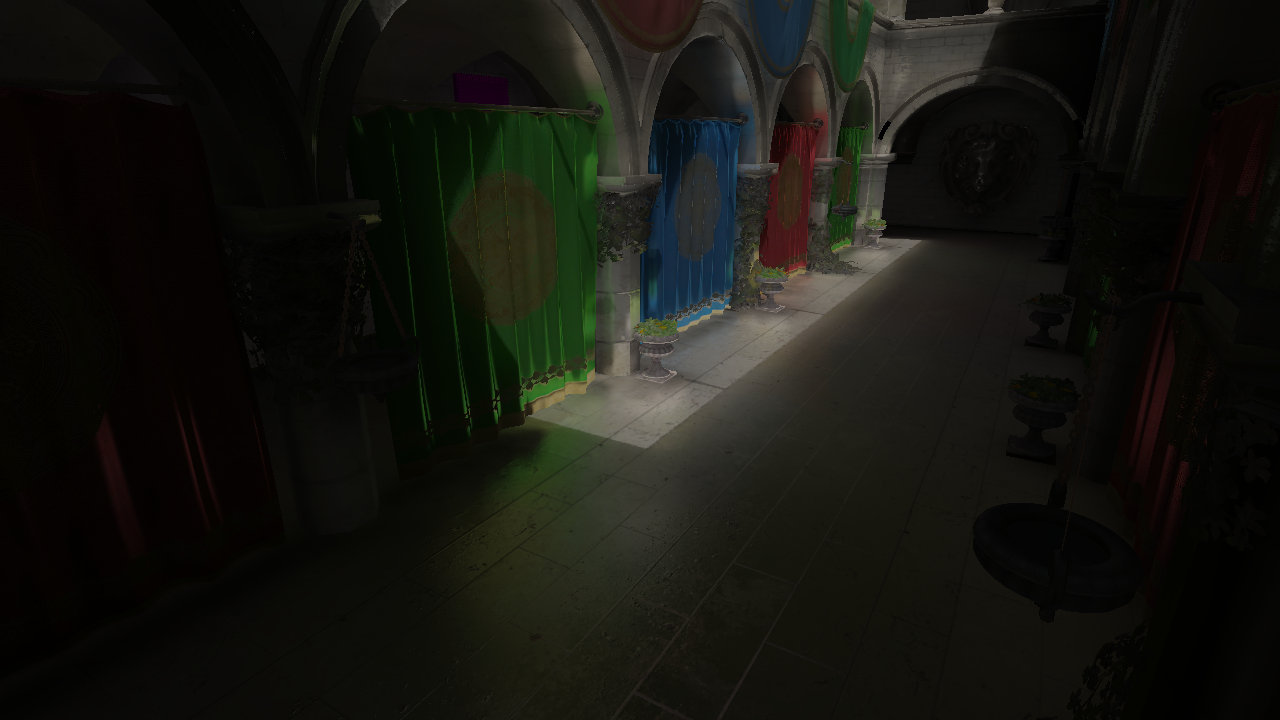
\includegraphics[width=\textwidth]{voxelwarp_off.png}
        \caption{Without voxel warping}
    \end{subfigure}
    ~
    \begin{subfigure}[t]{0.475\textwidth}
        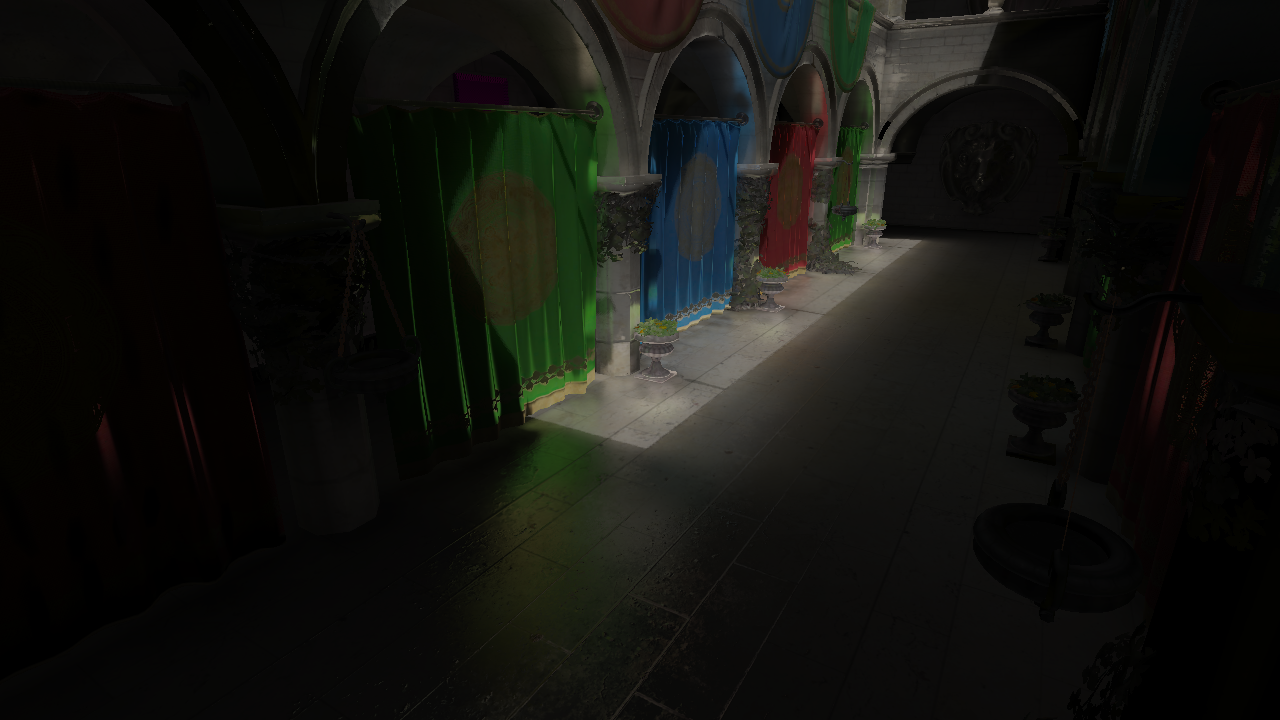
\includegraphics[width=\textwidth]{voxelwarp_on.png}
        \caption{With voxel warping}
    \end{subfigure}
    \caption{The voxel warping only has a small effect on lighting quality (the reflection of the green curtain is slightly more detailed).}
    \label{fig:results_voxelwarp}
\end{figure}

The second method of voxelization utilizes perspective projection to determine the voxel sizes. The motivation behind this is for voxel sizes to correspond to their respective sizes in screen space. The lighting quality for this approach is noticeably more detailed than with the warp function, as seen in Figure~\ref{fig:results_tesswarp}, however the temporal flickering issues are still apparent. With future work, we think this can be alleviated or eliminated.

\begin{figure}
    \centering
    \begin{subfigure}[t]{0.475\textwidth}
        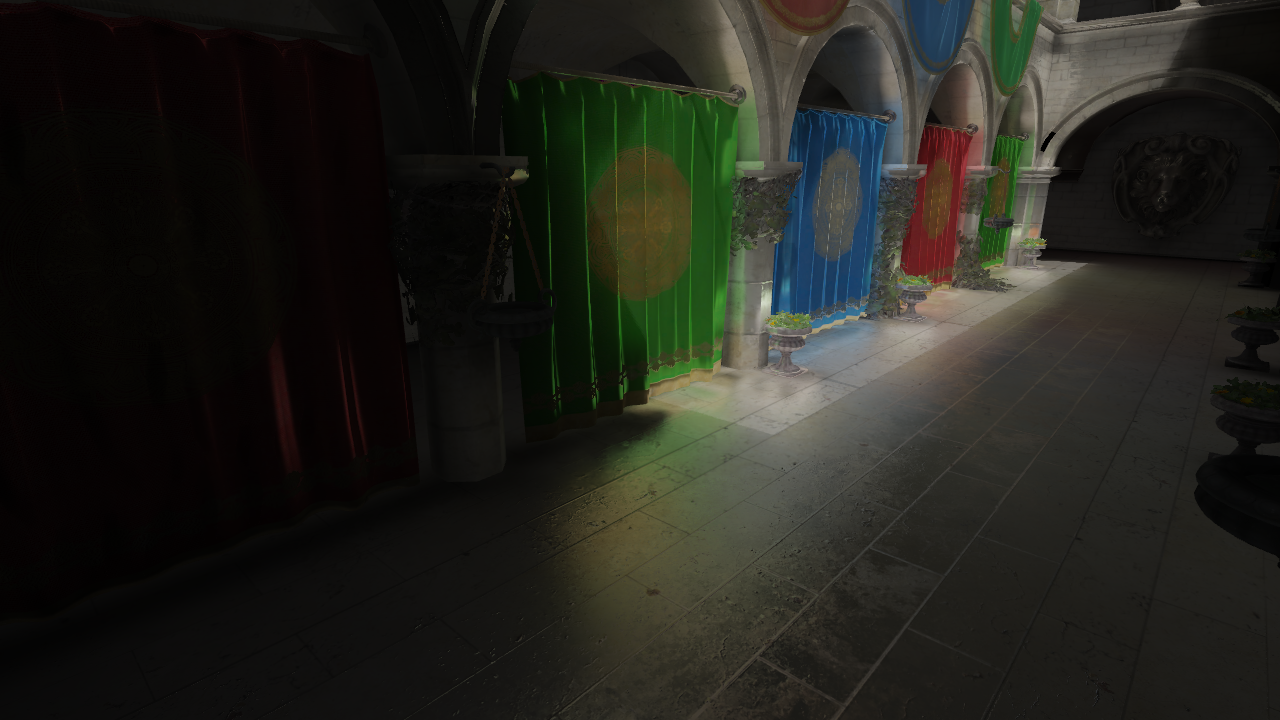
\includegraphics[width=\textwidth]{tesswarp_off.png}
        \caption{Without voxel warping}
    \end{subfigure}
    ~
    \begin{subfigure}[t]{0.475\textwidth}
        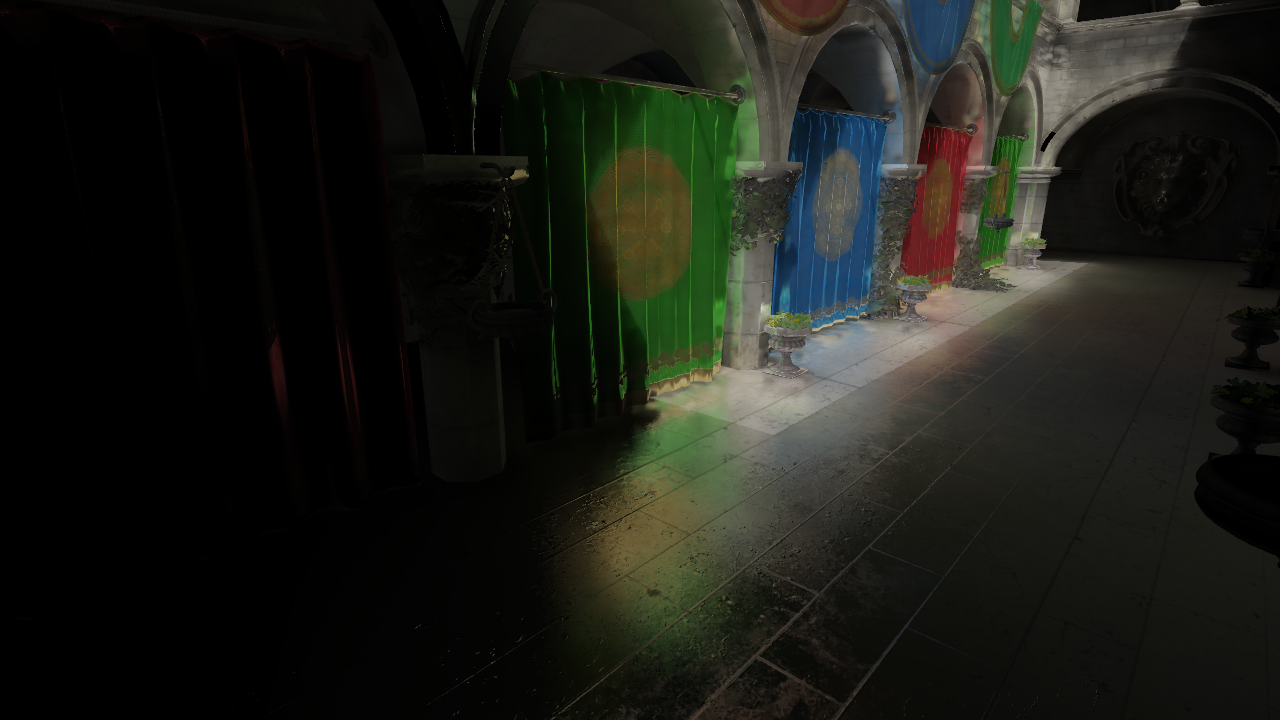
\includegraphics[width=\textwidth]{tesswarp_on.png}
        \caption{With voxel warping}
    \end{subfigure}
    \caption{The perspective voxel warping has a noticeable effect on lighting quality.}
    \label{fig:results_tesswarp}
\end{figure}
